\documentclass[10pt,letterpaper]{article}
\usepackage{float}
\usepackage{pslatex}
\usepackage{apacite}
\usepackage{graphicx}
\usepackage{ccn}
\usepackage{amssymb,amsmath,amsthm}
\newtheorem{assumption}{Assumption}

\usepackage{todonotes}
\newcommand{\rob}[1]{\todo[color=red!40]{Rob: #1}}
\newcommand{\aldo}[1]{\todo[color=yellow!40]{Aldo: #1}}

\title{Action Grammars: A Cognitive Model for Learning Temporal Abstractions}
 
\author{{\large \bf Robert Tjarko Lange (robert.lange17@imperial.ac.uk)} \\
  Einstein Center for Neurosciences Berlin, Chariteplatz 1, 10117, Berlin, Germany \AND {\large \bf Aldo Faisal (a.faisal@imperial.ac.uk)} \\
  Imperial College London, South Kensington Campus, London SW7 2AZ, United Kingdom}


\begin{document}

\maketitle


\section{Abstract}
{
\bf
Hierarchical Reinforcement Learning algorithms have successfully been applied to temporal credit assignment problems with sparse reward signals. State-of-the-art algorithms require manual specification of sub-task structures,  a sample inefficient exploration phase or lack semantic interpretability. Human infants, on the other hand, efficiently detect hierarchical sub-structures induced by their surroundings.
In this work we propose a cognitive-inspired Reinforcement Learning architecture which uses grammar induction to identify sub-goal policies. More specifically, by treating an on-policy trajectory as a sentence sampled from the policy-conditioned language of the environment, we identify hierarchical constituents with the help of unsupervised grammatical inference. The resulting set of temporal abstractions is called \textit{action grammars} \cite{Pastra_2012} and can be used to enable efficient imitation, transfer and online learning.
}
\begin{quote}
\small
\textbf{Keywords:} 
Decision Making; Reinforcement Learning; Computational Linguistics
\end{quote}

\section{Introduction}

%Human infants learn complex patterns in nature by observing role models and their behavior. 
Genetically inherited inductive biases enable human infants to infer hierarchical rule-based structures from language, visual input as as well as auditory stimuli \cite{Frank_2009, Marcus_2007}. Several MEG and fMRI studies provide evidence for a universal method of hierarchical language comprehension in the brain \cite{Frank_2018, Brennan_2016, Nelson_2017} as well as a parallelism to motor control \cite{Pastra_2012, Stout_2018}. By processing trajectories of an expert, the infant is able to learn policies over higher level sequences of low level control elements.
Inspired by these observations, this work proposes to overcome the problem of sub-structure discovery in Hierarchical Reinforcement Learning (HRL) by making use of grammatical inference. More specifically, the HRL agent uses grammar induction to extract hierarchical constituents from trajectory sentences. The proposed solution to the credit assignment problem is split into two alternating stages (see fig. \ref{fig:loop_ag}):

\begin{enumerate}
	\item \textbf{Grammar Learning}: Given episodic trajectories we treat the time-series of transitions as a sentence sampled from the language of the policy-conditioned environment. Using grammar induction algorithms \cite{Manning_1997} the agent extracts hierarchical constituents of the current policy. Based on the estimated production rules, temporally-extended actions are constructed which convey goal-driven syntactic meaning. The grammar can efficiently be inferred (linear time) and provides enhanced interpretability.
	\item \textbf{Action Learning}: Using the grammar-augmented action space, the agent acquires new value information by sampling reinforcement signals form the environment. They refine their action-value estimates using Semi-Markov Decision Process (SMDP) Q-Learning \cite{Bradtke_1995}. By operating at multiple time scales, the HRL agent is able to overcome difficulties in exploration and value information propagation. Afterwards, the agent samples simulated sentences by rolling out transitions from the improved policy.
\end{enumerate}

\begin{figure}
    \centering
    %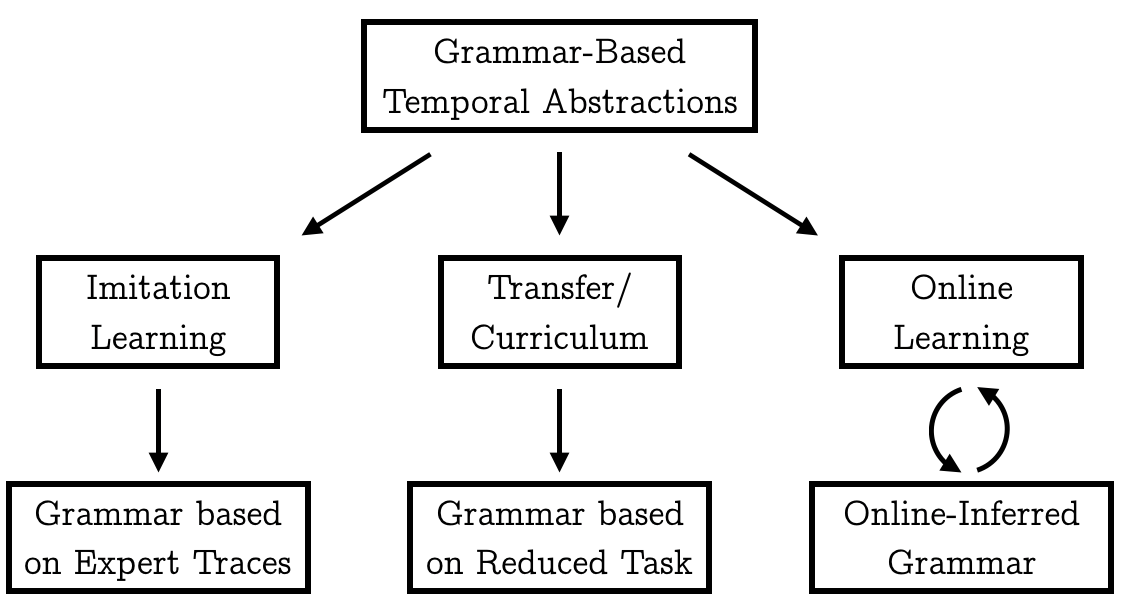
\includegraphics[width=\linewidth]{figures/concept_applications.png}
    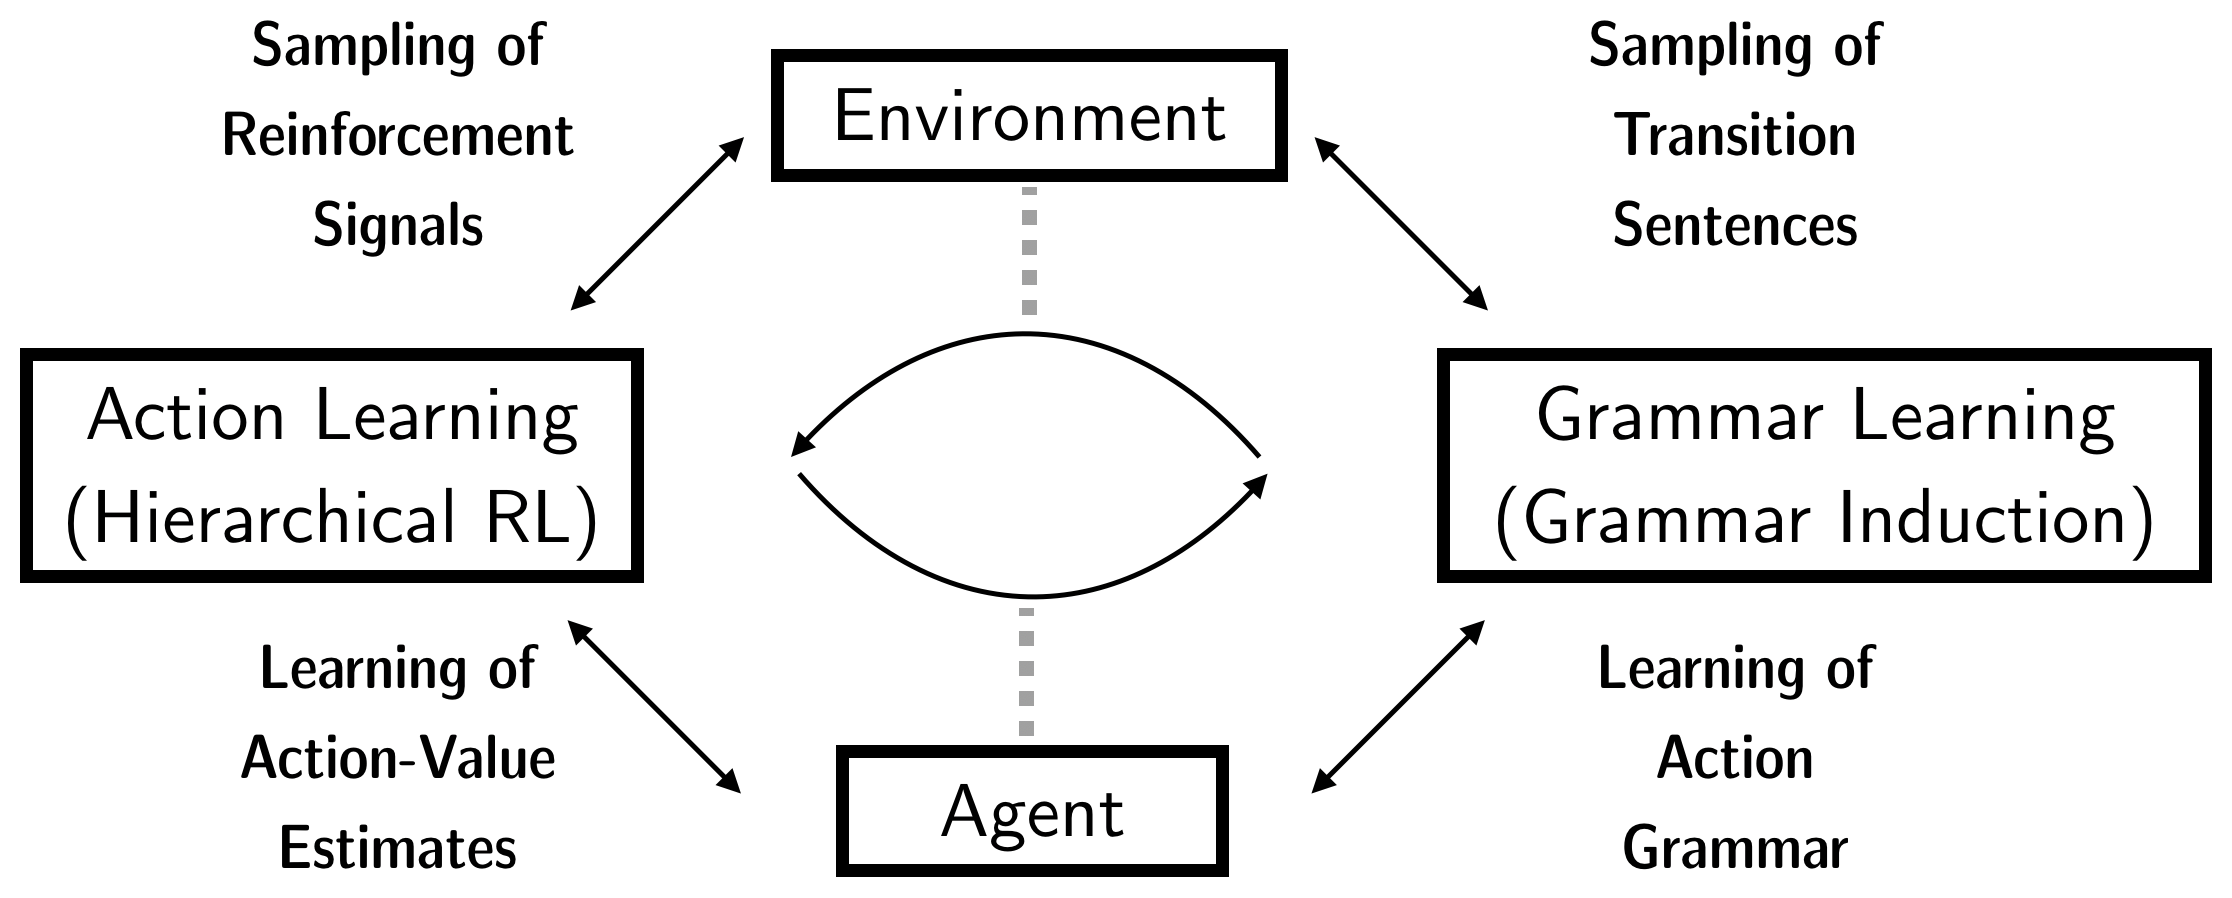
\includegraphics[width=\linewidth]{figures/concept_al_gl.png}
    \caption{Action grammars closed alternation loop.}
    \label{fig:loop_ag}
\end{figure}

By alternating between stages of grammar and action value learning the agent iteratively reflects on their behavior in semi-supervised manner. Thereby, they extract semantically meaningful sub-components and reduce the associated reward prediction error.
Our experiments highlight the effectiveness of the action grammars framework for imitation, curriculum and transfer learning given an expert policy rollout. Furthermore, we derive promising results for an online version which iteratively refines grammar and value estimates. 

\section{Background}

\textbf{Temporal Abstractions.} 
%Learning a policy over temporally-extended actions allows the HRL agent to combat the uncertainty induced by single time-step decision making. The agent overcomes exploration problems, by restricting their decision process in a syntactically meaningful way.
SMDPs extend Markov Decision Processes to account for not only reward and transition uncertainty but also time uncertainty. The time between individual decisions is modeled as a random variable, $\tau \in \mathbb{Z}_{++}$. The waiting time is characterized by the joint likelihood of transitioning from state $s \in \mathcal{S}$ to state $s'$ in $\tau$ time steps given action $m$ was pursued, $P(s', \tau| s, m)$. Thereby, SMDPs allow one to elegantly model the execution of actions which extend over multiple time-steps. A macro-action \cite{McGovern_1997}, $m \in \mathcal{M}$ specifies the sequential and deterministic execution of multiple ($\tau_m$) primitive actions. Let $r_{\tau_m} = \sum_{i=1}^{\tau_m} \gamma^{i-1} r_{t+i}$ denote the accumulated and discounted reward for executing a macro. Value estimates can then be updated using SMDP-Q-Learning \cite{Parr_1998a} in a model-free bootstrapping-based manner:
$$Q(s, m)_{k+1} = (1-\alpha) Q(s, m)_k + \alpha \left( r_{\tau_m} + \gamma^{\tau_m} \max_{m' \in \mathcal{M}} Q(s', m')_k \right)$$  
%In order to increase sample efficiency one can perform intra-macro updates for each state transition tuple $\{<s,a,r,s'>\}_{\tau_m}$ within the macro execution.
The DQN \cite{Mnih_2015} objective can then be adapted to the semi-Markov case:
$$L(\theta) := \mathbb{E} [(r_{\tau_m} + \gamma^{\tau_m} \max_{m' \in \mathcal{A} \cup \mathcal{M}} Q(s',m';\theta^-) - Q(s,m; \theta))^2] $$

The gradient with respect to the parameters is approximated by Monte Carlo samples from the experience replay (\citeA{Lin_1992}; ER) buffer $\{s,m,r_{\tau_m},s', \tau_m\} \sim D_{\mathcal{M}}$. The learning dynamics can be stabilized by making use of a target network and gradient clipping.

\textbf{Context-Free Grammars.} Given a start symbol $S$, a formal grammar $(\Sigma, \mathbb{N}, S, \mathcal{P})$ produces an output of strings. Production rules $\mathcal{P}$ map a set of non-terminal vocabulary $\mathbb{N}$ either to another non-terminal or terminal string within the terminal vocabulary $\Sigma$.
Context-free grammars (CFG) \cite{Chomsky_1959a} constrain the set of productions to either map from one-to-one, one-to-none or one-to-many. A non-branching and loop-free CFG is called a straight-line grammar. Given a sample of sentences, grammar induction infers a consistent language grammar.
Sequitur \cite{Manning_1997} sequentially reads in all symbols and collects repeating subsequences of symbols into a production rule. Therewhile, the final encoded string is only allowed to have unique bigrams and inferred production rules must be used more than once in the derivation of the string.
In order to overcome Sequitur's problem of noise overfitting, $k$-Sequitur \cite{Stout_2018} has been proposed. Instead of replacing a bigram with a rule if the bigram occurs twice, it has to occur at least $k$ times. As $k$ increases the grammar becomes less prone to overfitting and the resulting grammar is more parsimonious in terms of production rules. 
%Lexis \cite{Siyari_2016b} provides an optimization-based alternative which iteratively constructs a directed acyclic graph (DAG). Starting from a trivial graph which connects a set of target sentences with the set of elements in the terminal vocabulary, the Lexis-DAG is constructed by adding intermediate nodes. Again, this problem by itself is NP-hard. G-Lexis, the greedy algorithmic implementation, searches for substrings that will lead to a maximal reduction in the cost, when added as new intermediate node.

\section{Context-Free Action Grammars}

Action sequences as well as communication convey goal-directed semantic meaning. They consist of hierarchical structures and are conditioned on the environment in which they are uttered. 
Furthermore, many real world problems require a hierarchy of subgoal achievements which increase in sequential difficulty and timescale.
A trajectory obtained from traversing the current policy $\pi$ can be viewed as a sample from the language generated by the policy-specific grammar, $L(\pi|E)$. Let the terminal vocabulary $\Sigma$ consist of the primitive action space $\mathcal{A}$, hence $\Sigma = \mathcal{A}$. We denote  $\vartheta^i \sim L(\pi|E)$ for $i = 1, \dots N_g$ trajectories. Given a set of trajectories, a CFG estimate $\hat{G}$ can be inferred and the resulting production rules transformed into macro-actions $\mathcal{M}^{\hat{G}}$ by recursively flattening the non-terminals. The action space of the action grammar HRL agent is then augmented such that $\mathcal{A}^{\hat{G}} = \mathcal{A} \cup \mathcal{M}^{\hat{G}}$. Depending on the generating policy of the compressed traces, we propose several grammar-based HRL agents.

\textbf{Expert \& Transfer Grammars.} If the traces $\vartheta^i$ are sampled from the language $L(\pi^\star|E)$ generated by the optimal policy, the agent can use the resulting grammar macros in an imitation learning setting. Before the onset of the first value learning stage, the action space is augmented with the optimal productions. Furthermore, an agent faced with learning a curriculum of tasks can make use of the optimal grammar of an easier solved task. Skills universal to all tasks do not have to be re-learned at every stage. Instead, the inferred optimal grammar provides an effective knowledge structure which accelerates the agents learning process.

\textbf{Online Inferred Grammars.} If an episode successfully terminated, the grammar inference process identifies repeating sub-goal achieving patterns. We hypothesize that by extracting action grammar sub-sequences, one compresses the temporal dimension of the credit assignment problem. After each grammar compression step, the action space is augmented with a new set of grammar macros. The previous set becomes inactive. 
In order to preserve value estimates between updates, we propose three solutions:
(1) \textit{Transfer learning} (\citeA{Oquab_2014}, see fig. \ref{fig:online_ag_dqn}): To accommodate the variable set of grammar-inferred skills, the size of the DQN output layer has to be updated. Transferring the value-relevant feature detectors between action space augmentation, allows the agent to use the previously learned value characteristics.
(2) \textit{Grammar ER Buffer}: It is necessary to maintain a separate buffer system in order to store transition tuples specific to previously inferred macro-actions. At any given point the agent can only sample macro transitions which are associated with the currently active set of grammar macros. Thereby, sample efficiency is increased once a grammar macro is repeatedly inferred.
(3) \textit{Intra-Macro Updates}: During the execution of a macro-action, one stores the overall macro transition tuple $<s_t,m_t,r_{t +\tau_m}, s_{t +\tau_m +1}, \tau_m, "on">$ as well as the individual transitions $\{<s_i,a_i,r_i, s_{i+1}, 1, "on">\}_{i=t}^{t + \tau_m}$. Thereby the agent is able to exploit all gathered transition experiences throughout the overall learning process.

\begin{figure}[H]
    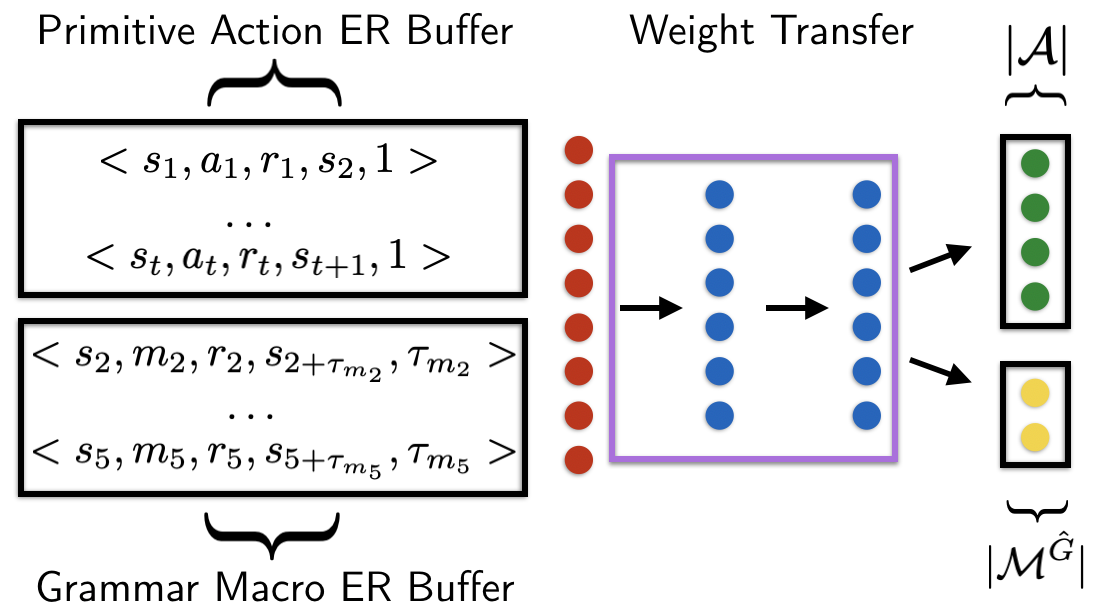
\includegraphics[width=\linewidth]{figures/ag_dqn_buffer}
    \caption{\textbf{Left.} Grammar Experience Replay Buffer \textbf{Right.} Grammar-DQN with adaptive output head.}
  \label{fig:online_ag_dqn}
\end{figure}
    
The length of the sampled trace is going to increase or decrease over the course of the learning procedure. The regularization parameter of the $k$-Sequitur grammar inference algorithm has to be adapted accordingly.

\section{Experiments}

The goal of the following experiments is to answer the following questions: (1) Does a grammar learned from optimal policy rollouts allow for rapid imitation learning? (2) Can CFG grammars be used in order to enhance curriculum learning by the means of transferring previously learned action grammars? (3) Is online grammar inference and action space adaptation able to structure the exploration process of the HRL agent?
In order to illustrate our results we choose the general $N$-disk Towers of Hanoi (ToH) environment (see fig. \ref{fig:hanoi}) as well as a hierarchically structured gridworld task (see fig. \ref{fig:gridworld}).

Solving the $N$-disk ToH problem requires the agent to identify a hierarchical and recursive principle. By moving $n-1$ disks onto an auxiliary pole and the $n$-th disk onto the target pole, the agent is able solve the sparse reward problem. Since such a routine can easily be formulated within a grammar parse tree, we hypothesize that the action grammars framework might provide an efficient solution.

%The agent maximizes their expected cumulative discounted reward by reaching the final state $(3)_{i=1}^N$ as quickly as possible. The problem is formulated as a sparse long-term credit assignment problematic. The size of the state space, on the other hand, grows exponentially, $|S| = 3^N$ (all possible allowed orderings), and the optimal number of moves to solve this game is given by $2^N - 1$. 

\begin{figure}[H]
    \centering
    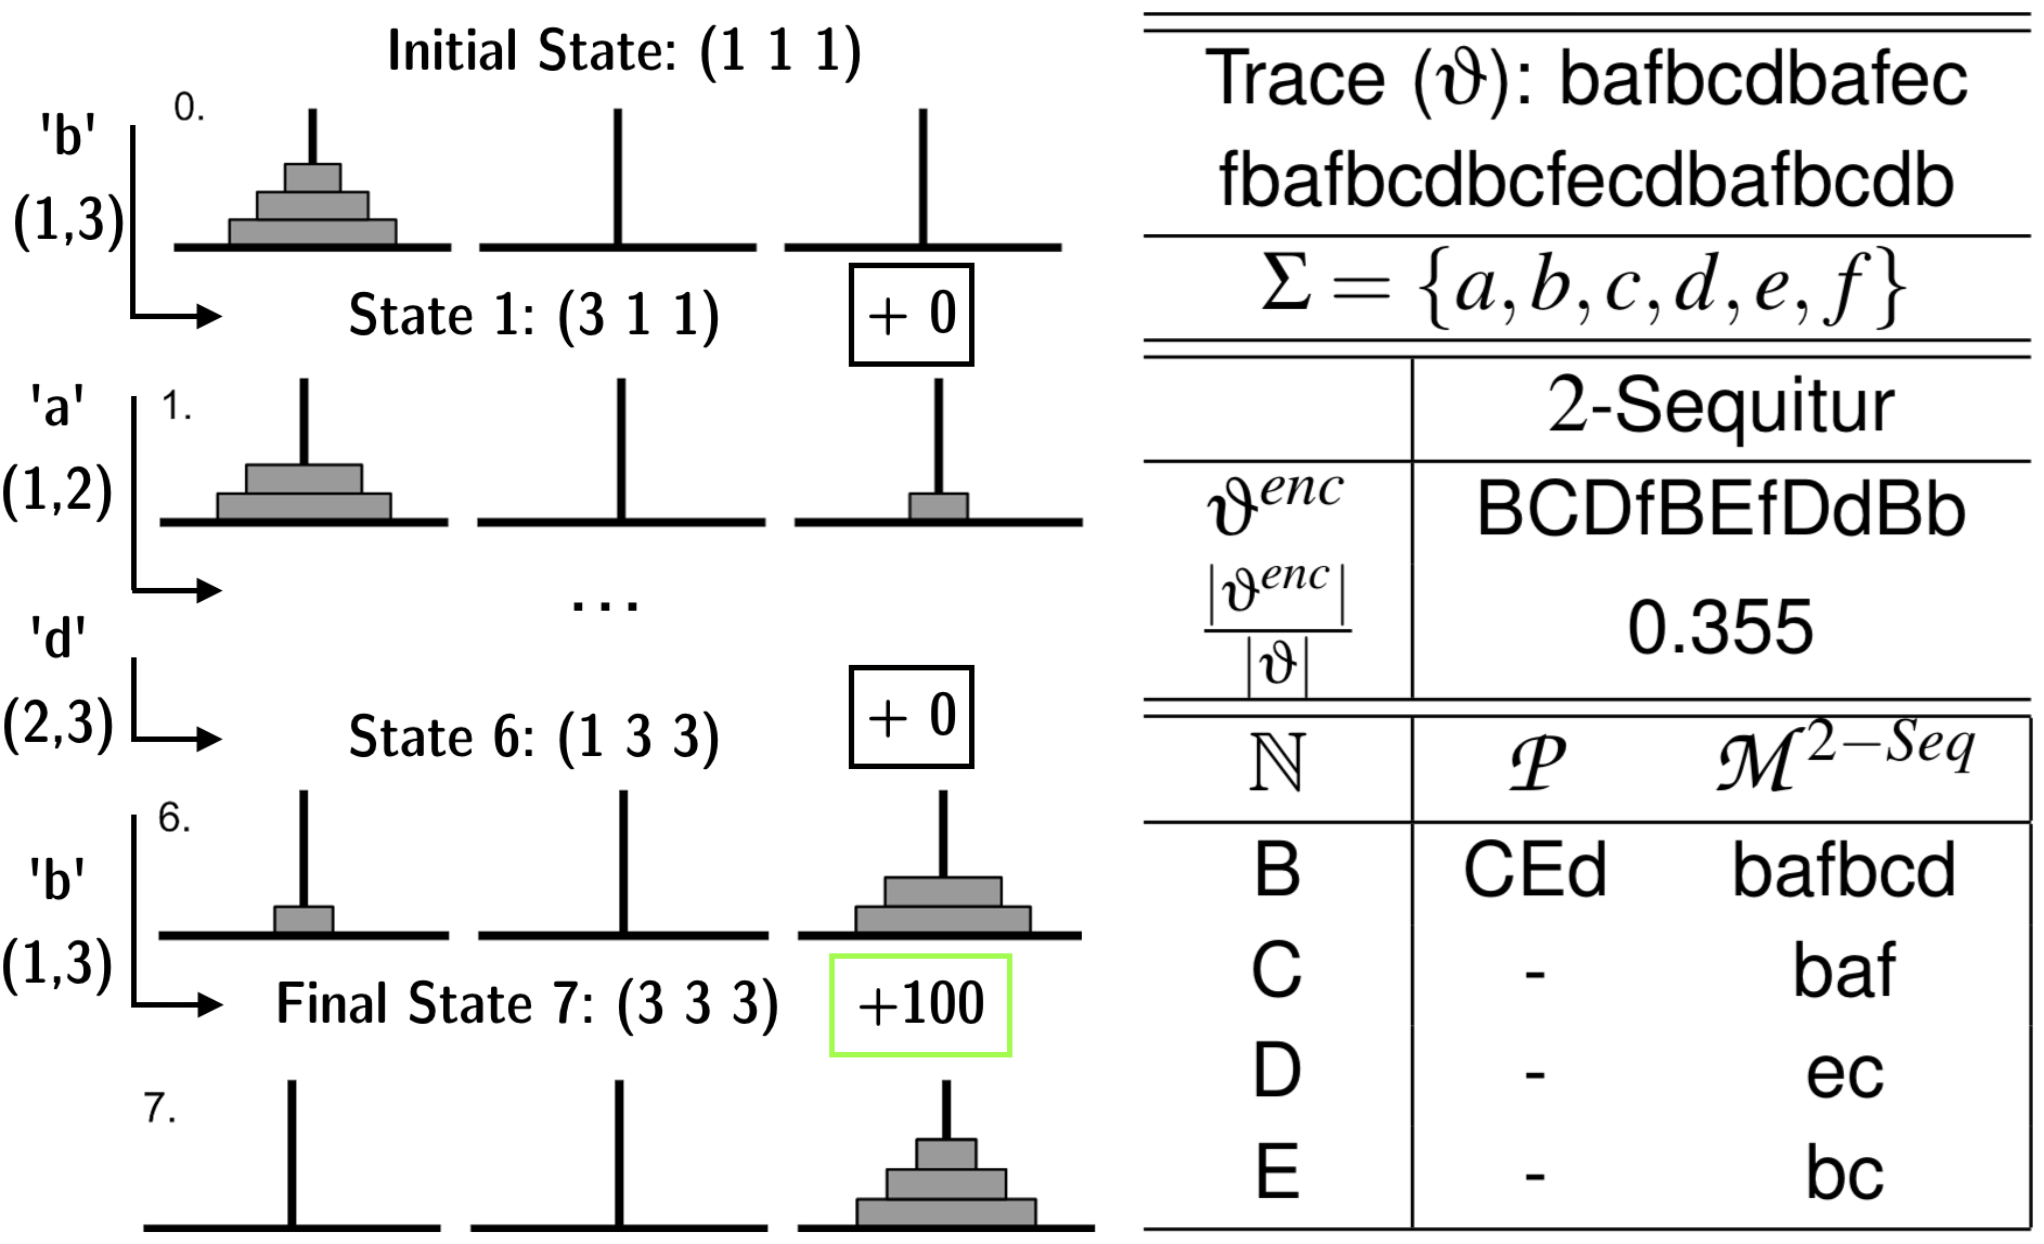
\includegraphics[width=\linewidth]{figures/hanoi_grammar.png}
    \caption{\textbf{Left.} Sparse Reward RL Formulation of the ToH Problem. \textbf{Right.} 2-Sequitur ToH (5 disks) Grammar-Macros.}
    \label{fig:hanoi}
 \end{figure}
 
 \begin{figure}[H]
    \centering
    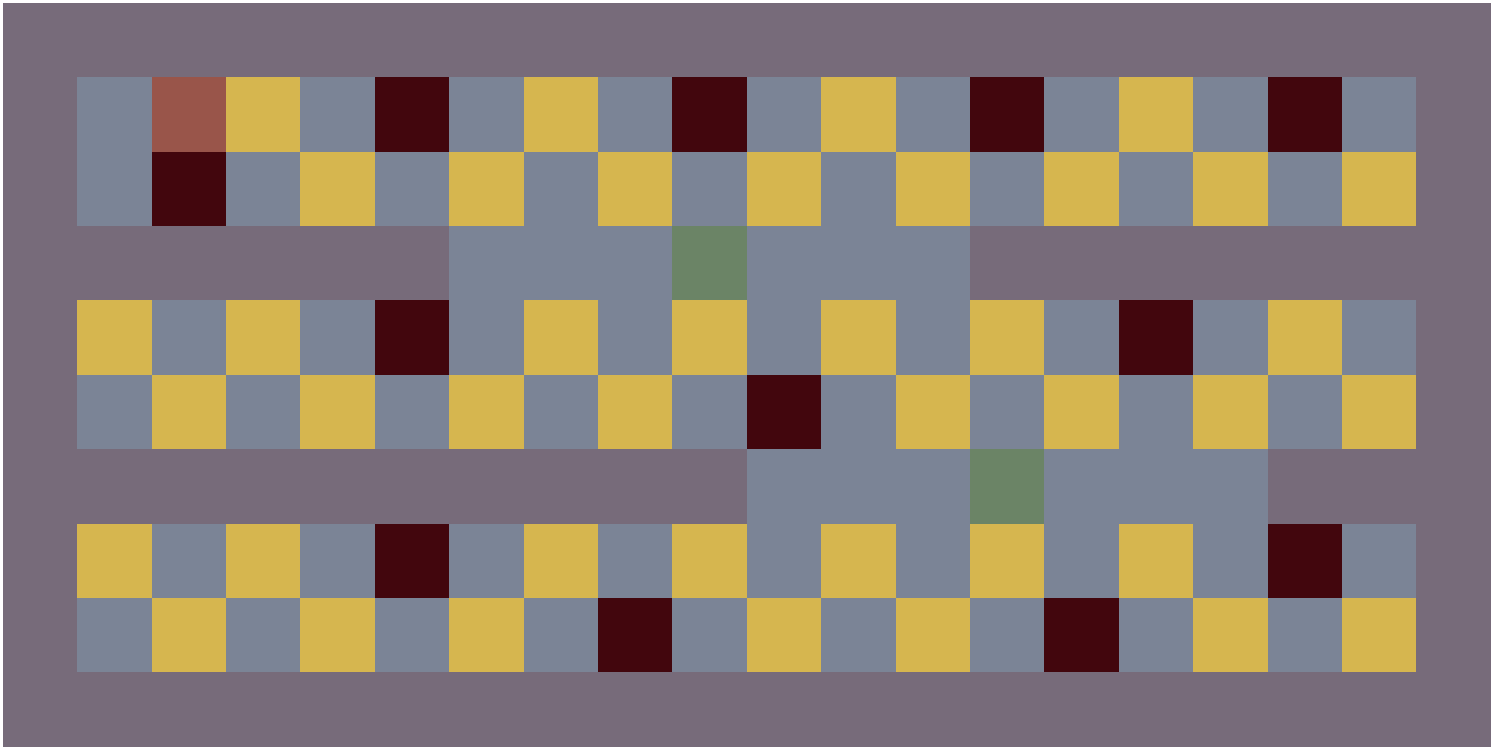
\includegraphics[width=0.75\linewidth]{figures/gridworld}
    \caption{Hierarchically-Structured Grid World Environment.}
    \label{fig:gridworld}
 \end{figure}
 
The gridworld, on the other hand, provides a non-sparse reward design. The agent (red) has to avoid poisonous items (black) and collect food (yellow). Hence, the agent is required to solve a large set of individually smaller subtasks. Finally, the agent has to avoid a terminal collision with the moving blocks (green), whereas the ToH environment rewards the fastest solution. 
 
%-----------------------------------
\textbf{Learning with Expert \& Transfer Grammars.} The right-hand side of figure \ref{fig:hanoi} shows the grammar and resulting macros inferred from a trace of the optimal policy 5-disk ToH problem using the 2-Sequitur. The flattened production rule $B \to CEd \to bafbcd$ captures the recursive nature learned by the grammar. $C \to baf$ moves two disks on the auxiliary pole, while $E \to bc$ moves a third disk from source to target pole and one disk back onto the source pole. The Expert Grammar HRL agent's action space is augmented as follows:
$$\mathcal{A}^{\hat{G}} = \mathcal{A} \cup \mathcal{M}^{2-Seq} = \mathcal{A} \cup \{bafbcd, baf, ec, bc\}$$

Figure \ref{fig:expert_grammar_toh} displays learning results for different SMDP-Q-Learning agents with macro-actions defined by the production rules inferred from a single trace of the optimal policy. 
\begin{figure}[H]
\minipage{0.51\linewidth}
  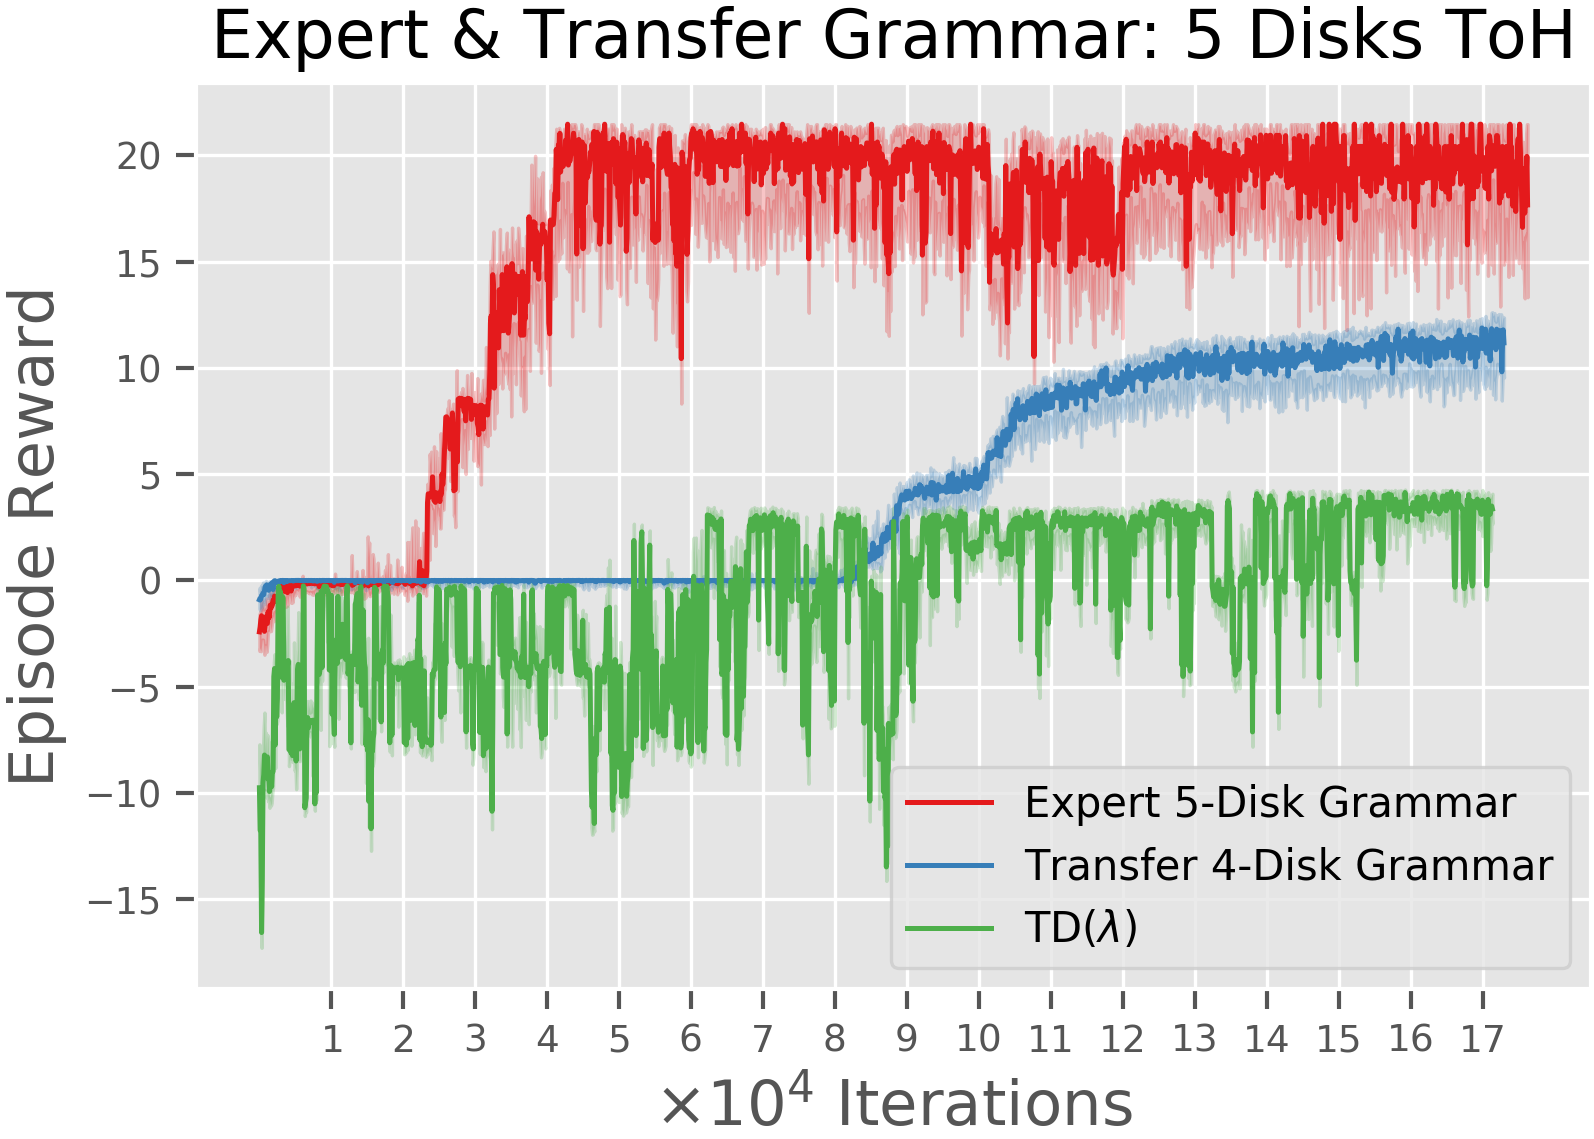
\includegraphics[width=\linewidth]{figures/hanoi_5_learning_curve}
\endminipage\hfill
\minipage{0.49\linewidth}
  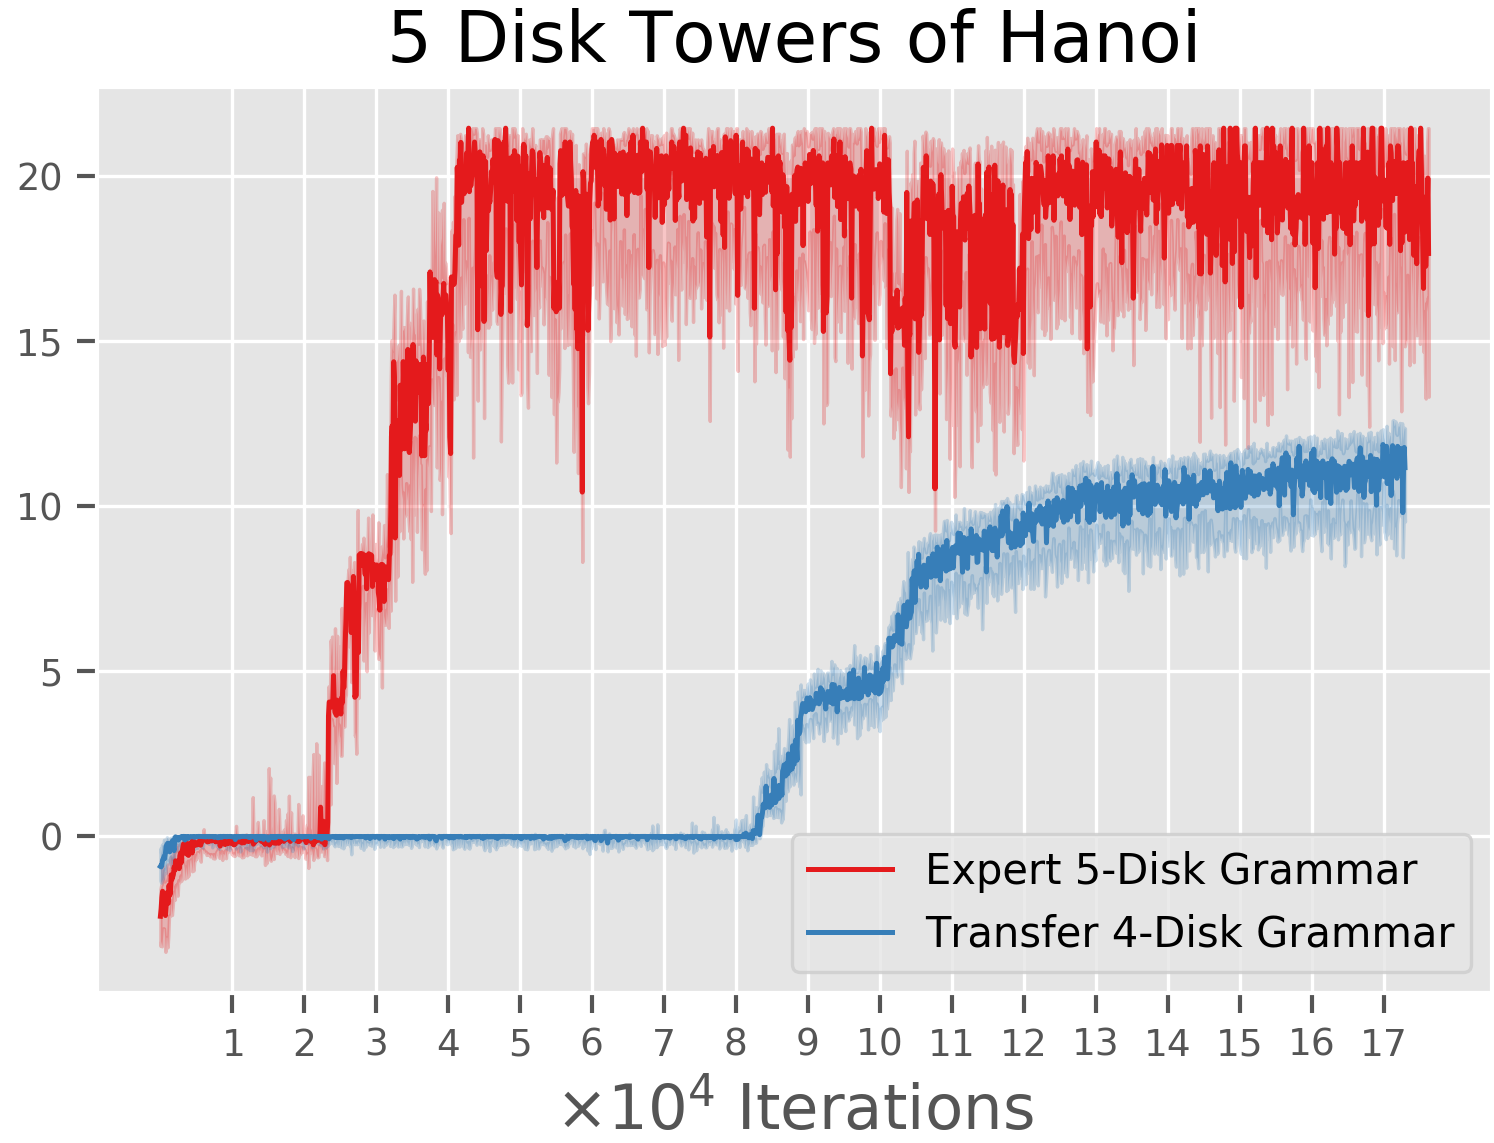
\includegraphics[width=\linewidth]{figures/hanoi_6_learning_curve}
\endminipage\hfill
\caption{Expert \& Transfer Grammar (\textit{ToH}): \textbf{Left.} 5 Disk Environment. \textbf{Right.} 6 Disk Environment. Averaged over 5 random seed. Median, 10th and 90th percentile.}
\label{fig:expert_grammar_toh}
\end{figure}

The grammar macros accelerate the learning progress of the agent. Furthermore, the variance of policy rollouts is reduced due to an increased robustness related to the temporal compression of the sequential problem.
Finally, the Transfer Grammar agent is capable of transferring the knowledge distilled in a simpler optimal grammar(4 disks) to a more complex setting (6 disks).  

\begin{figure}[H]
\minipage{0.51\linewidth}
  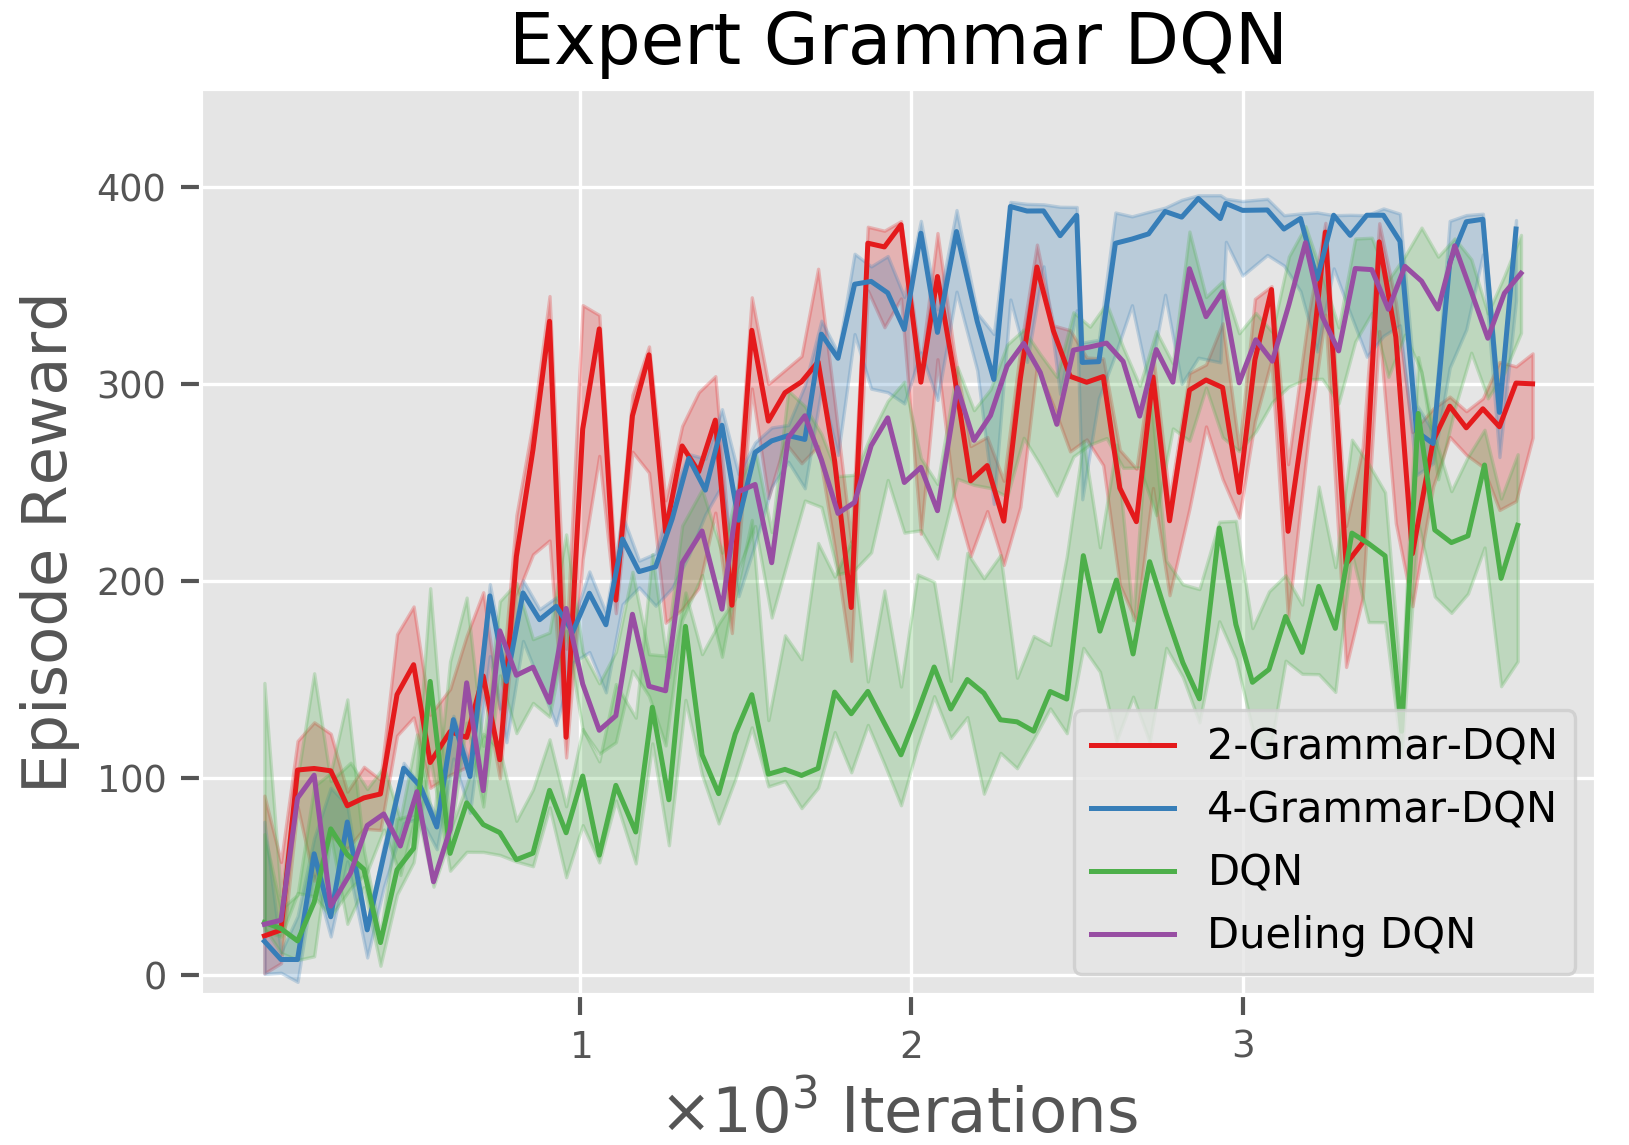
\includegraphics[width=\linewidth]{figures/grammar_dqn_gridworld_expert}
\endminipage\hfill
\minipage{0.49\linewidth}
  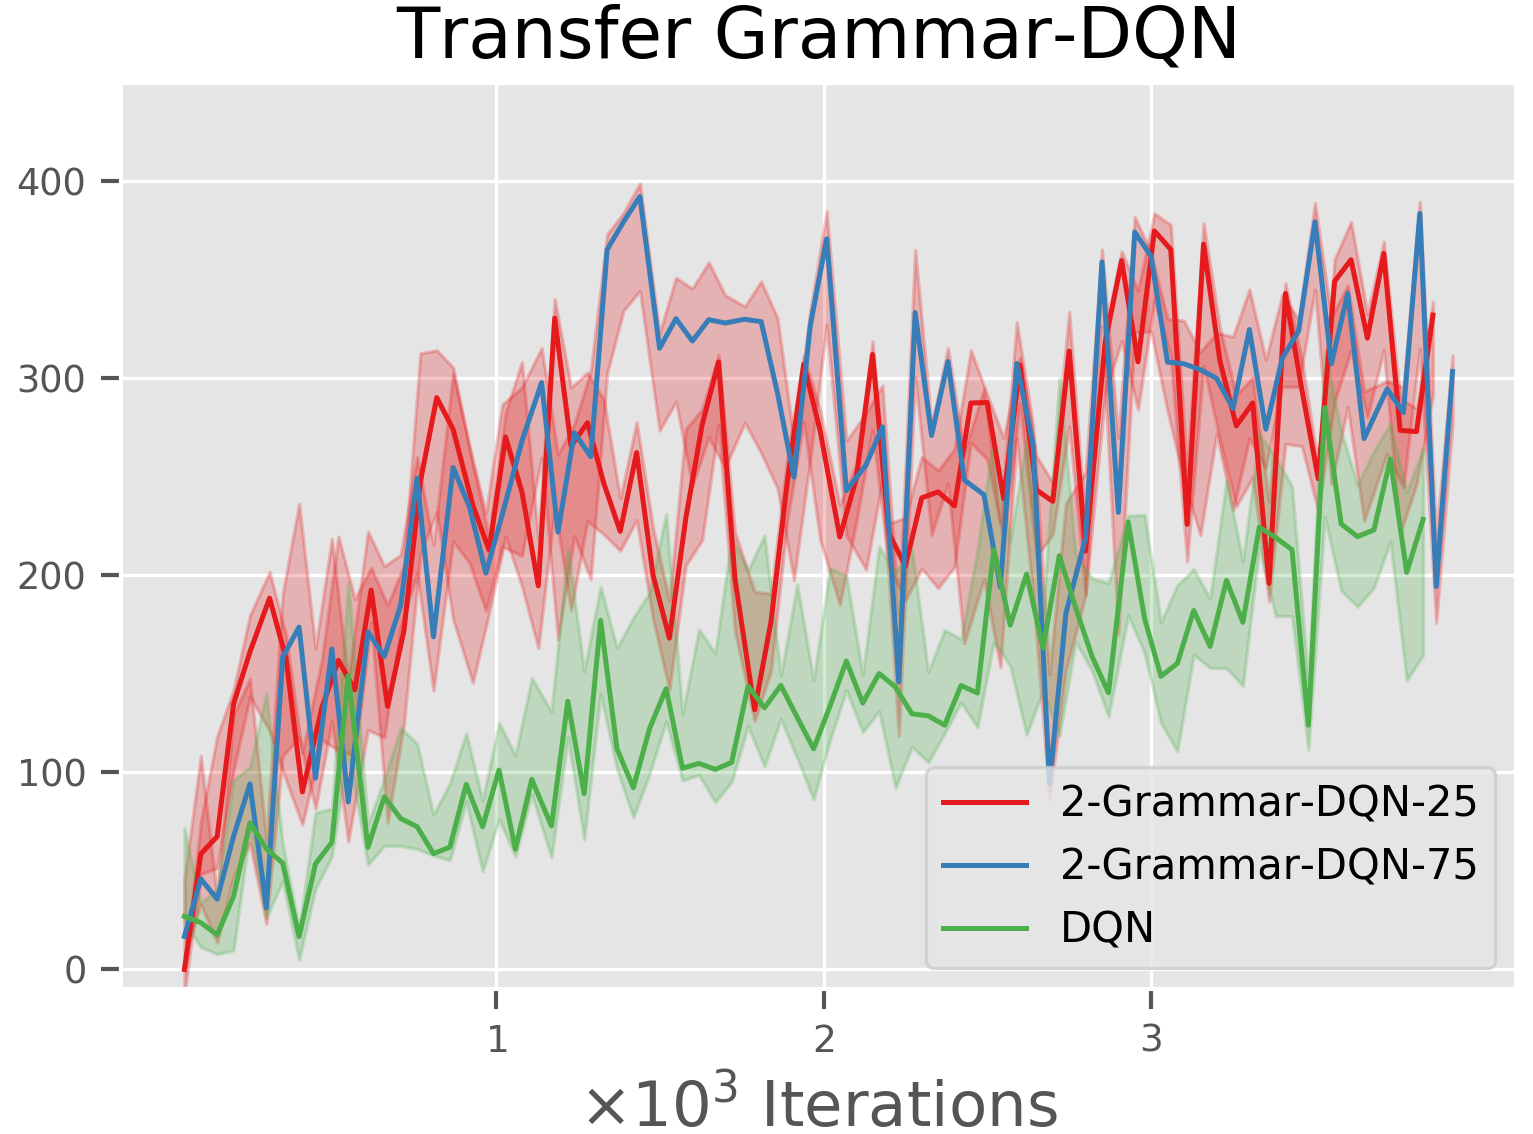
\includegraphics[width=\linewidth]{figures/grammar_dqn_gridworld_transfer}
\endminipage\hfill
\caption{Expert \& Transfer Grammar (\textit{Gridworld}): \textbf{Left.} Expert Grammar. \textbf{Right.} Transfer Grammar. Averaged over 5 random seed. Median, 10th and 90th percentile.}
\label{fig:expert_grammar_grid}
\end{figure}

The gridworld Grammar-DQN agent (see fig. \ref{fig:expert_grammar_grid}) again infers a set of macro-actions from a single expert rollout. Afterwards, the output layer and action space are augmented. The fixed architecture of the DQN is a two-layer 128 hidden units multi-layer perceptron trained using Adam \cite{Kingma_2014} with a batch-size of 32.
The two Expert Grammar-DQN agents differ in the amount of macro-actions (top two and four most used productions in the encoded policy trace) inferred with 2-Sequitur on a converged DQN agent rollout. Again, the expert grammar-endorsed agent is significantly accelerated in their initial learning progress.
The two Transfer Grammar-DQN agents, on the other hand, infer a set of two grammar macros from a single sub-optimal separate DQN agent's (trained for 25 or 75 episodes) policy rollout. Our experiments show, that even with noisy non-optimal rollouts the grammar agents are able to exploit the inferred structure of the environment.

%-----------------------------------
\textbf{Learning with Online Inferred Grammars.} Figure \ref{fig:online_grammar} displays the results of the online grammar macro inference framework for the 4 disks ToH problem as well as the gridworld task.\rob{Add figure and describe results}

\begin{figure}[H]
\minipage{0.51\linewidth}
  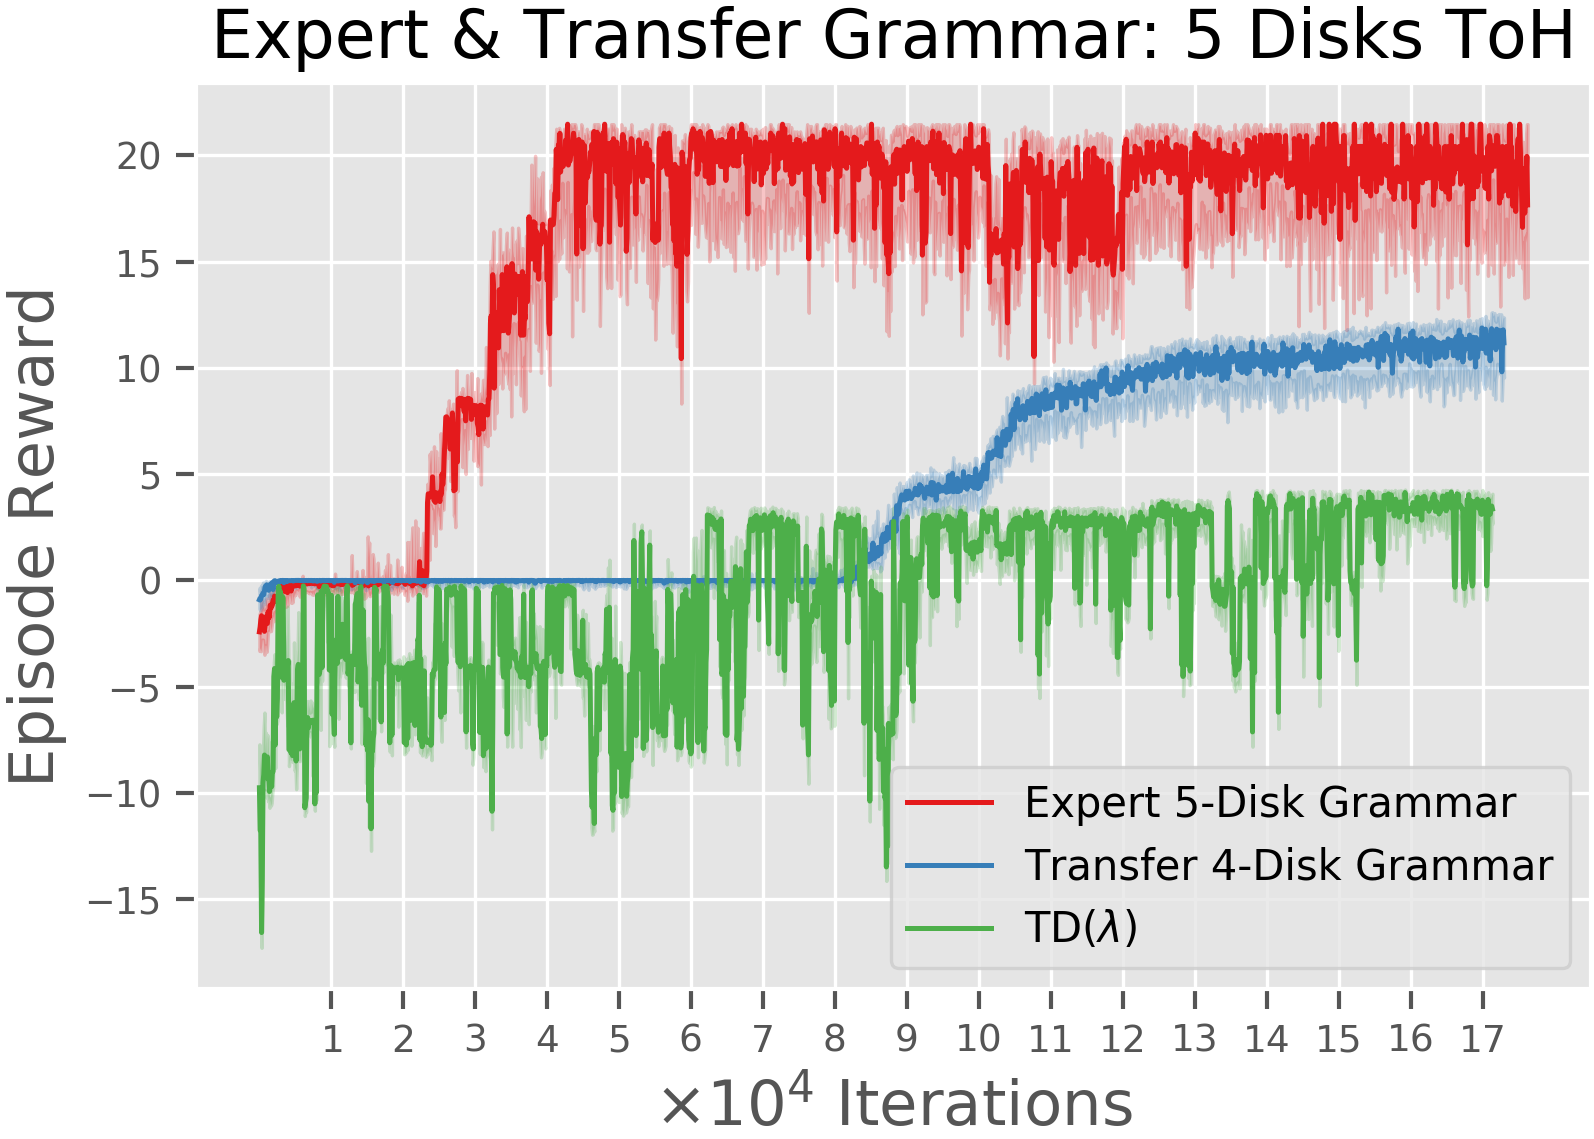
\includegraphics[width=\linewidth]{figures/hanoi_5_learning_curve}
\endminipage\hfill
\minipage{0.49\linewidth}
  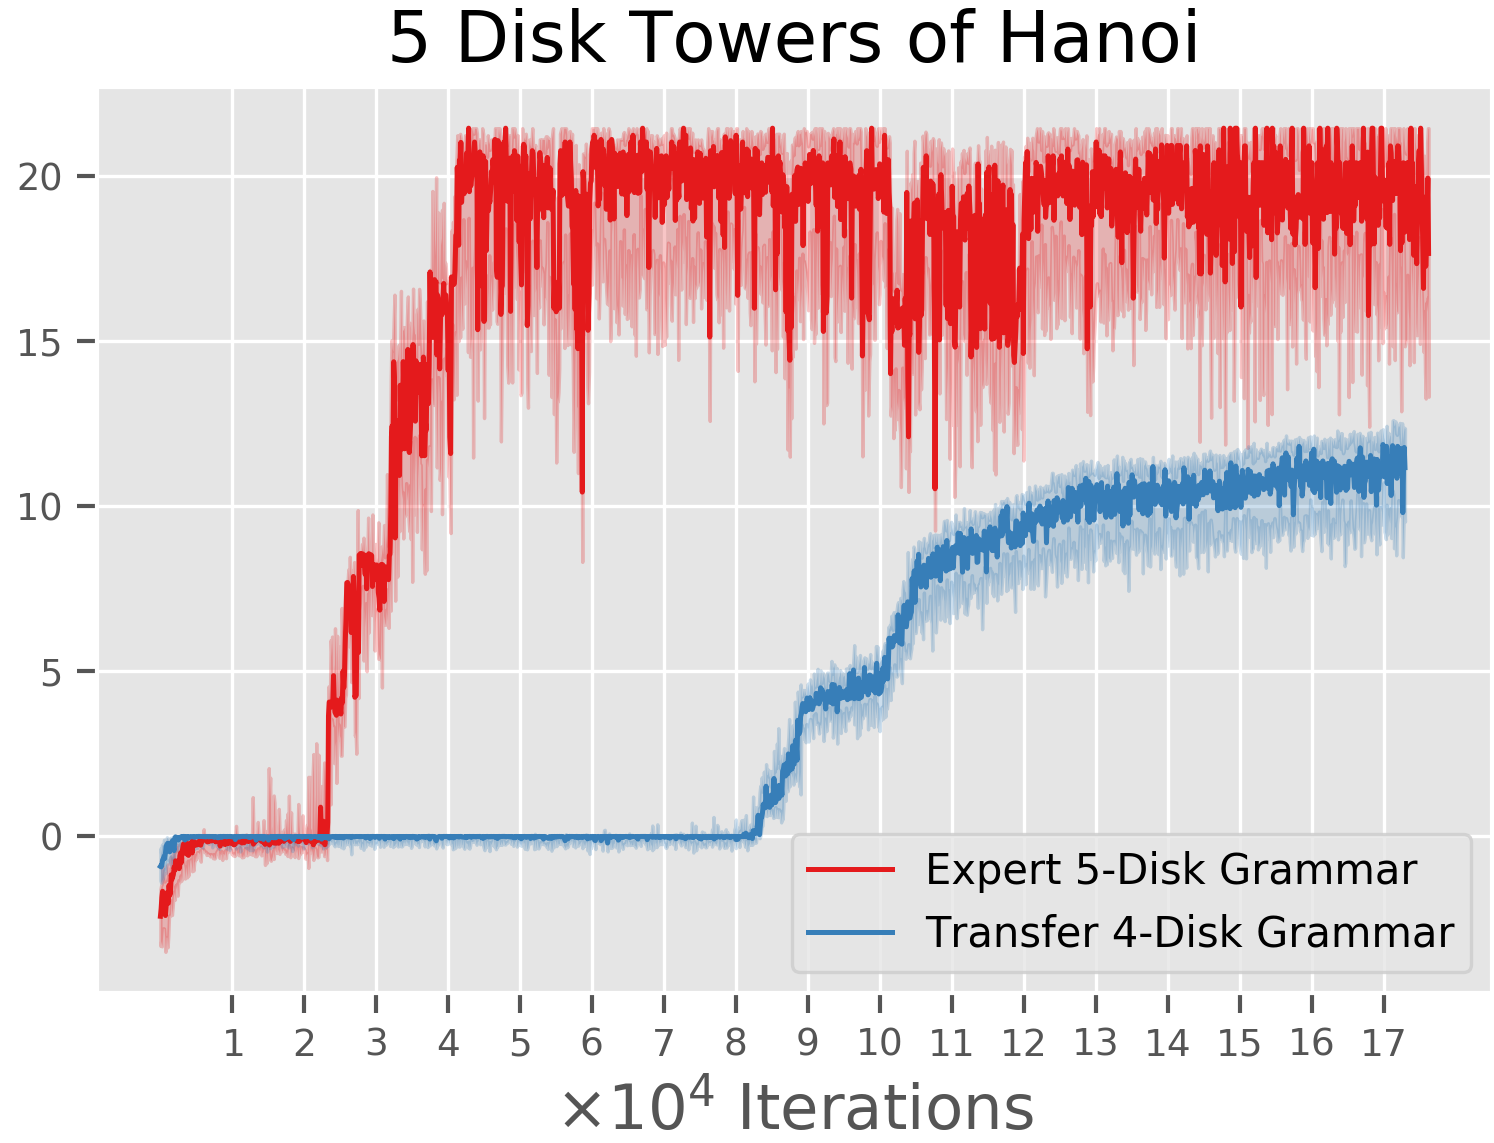
\includegraphics[width=\linewidth]{figures/hanoi_6_learning_curve}
\endminipage\hfill
\caption{Online Grammar: \textbf{Left.} 4 Disk ToH Environment. \textbf{Right.} Gridworld Grammar DQN. Averaged over 5 random seed. Median, 10th and 90th percentile.}
\label{fig:online_grammar}
\end{figure}

We experiment with a linear decaying scheme in order to assure that an appropriate amount of productions are inferred.

\section{Conclusion}

Formal grammars do not only provide a powerful framework for studying language. Inspired by hierarchical parse trees of sequential behavior, we have derived a cognitive decision making framework which exploits grammatical inference to identify temporally-extended actions.
Our preliminary contributions are the following:
%
(1) CFG-based HRL agents provide efficient and interpretable solutions to imitation and transfer learning tasks.
%
(2) Alternating between grammar updates and learning action values is an effective method to learn an optimal grammar as well as an optimal policy online.

In future work we are interested in exploring stochastic grammars as well as their incorporation into model-based RL approaches. Furthermore, we intend to further analyze the relationship between grammar inference hyperparameters as well as exploration in HRL.
Ultimately, we envision a dictionary of action which provides an expandable library of skills for agents which act in diverse naturalistic environments. This could provide a mayor contribution to a key endeavor in general artificial intelligence: Life-long learning.

\newpage
\bibliographystyle{apacite}

\setlength{\bibleftmargin}{.125in}
\setlength{\bibindent}{-\bibleftmargin}

\bibliography{HRL}


\end{document}
